
\subsection{Constraints from the Higgs potential}\label{sec:2a}

In order to represent a viable model, the potential (\ref{potential}) must be bounded from below
and must have a neutral, not charge-breaking vacuum.
The former requirement leads to the well-known restrictions on the free parameters of the model:
\begin{equation}
\lambda_1>0,\ \  \lambda_2>0,\ \ 
2\sqrt{\lambda_1\lambda_2}+\lambda_3>0,\ \ 
2\sqrt{\lambda_1\lambda_2}+\lambda_3+\lambda_4 - |\lambda_5|>0\,.
\end{equation}
The absence of the charge-breaking vacuum is guaranteed if one assumes
\begin{equation}
\lambda_4 - |\lambda_5| < 0\,. \label{lam45-condition}
\end{equation}
This is a sufficient but not necessary condition for the vacuum to be neutral.
A neutral vacuum can also be achieved for positive $\lambda_4 - |\lambda_5|$ with appropriate
$m_1^2$ and $m_2^2$. However in this case the lightest DM candidate will be the charged scalar.
Condition (\ref{lam45-condition}) avoids this situation as well.

Once these restrictions are applied, the vacuum is neutral, and one can calculate the masses of the physical Higgs bosons.
In addition to the SM-like scalar $H$, one gets charged $h^\pm$ and neutral $h_1, h_2$ scalars. 
It is well known that the two neutral scalars of the i2HDM have opposite $CP$-parities, but it is impossible 
to unambigously assign which of them is $CP$-even and which is $CP$-odd.
In the absence of any suitable vertex, the model has two $CP$-symmetries, $h_1 \to h_1, h_2 \to -h_2$ and
$h_1 \to -h_1, h_2 \to h_2$, which get interchanged upon basis change $\phi_2 \to i \phi_2$. 
Either can be used as ``\textit{the $CP$-symmetry}'' of the model, 
making the specification of the $CP$ properties of $h_1$ and $h_2$ a basis dependent statement. 
Therefore, we denote the two neutral inert scalar masses as $M_{h_1} < M_{h_2}$, without specifying which is scalar and pseudoscalar.
The masses of the physical scalars are 
\begin{eqnarray}
&&M_H^2 = 2 \lambda_1 v^2 = 2m_1^2\,,\qquad
M_{h^+}^2 = {1\over 2} \lambda_3 v^2 - m_2^2\,,\nonumber\\
&&M_{h_1}^2 = {1\over 2}(\lambda_3 +\lambda_4 - |\lambda_5|) v^2 - m_2^2\,,\qquad
M_{h_2}^2 = {1\over 2}(\lambda_3 +\lambda_4 + |\lambda_5|) v^2 - m_2^2 \ >M_{h_1}^2\,.\label{masses}
\end{eqnarray}
The mass differences, written as
\begin{equation}
M_{h_2}^2 - M_{h_1}^2 = |\lambda_5| v^2\,,\quad 
M_{h^+}^2 - M_{h_1}^2 = -(\lambda_4 - |\lambda_5|) v^2/2\,,
\end{equation}
highlight the role of the parameters $\lambda_4$ and $\lambda_5$ and are consistent with (\ref{lam45-condition}).
It should also be stressed that the parameters $\lambda_1$ and $m_1^2$ correspond to the Higgs potential in the SM, and can thus be fixed by the values of the VEV and Higgs mass.

One also notices that the sign of $\lambda_5$ is phenomenologically irrelevant: 
flipping the sign of $\lambda_5$ would only lead to swapping the $CP$-parities
of the inert neutral scalars, which are unobservable anyway.
In order to eliminate double-counting, we make the standard choice of $\lambda_5 < 0$,
and introduce the shorthand notation $\lambda_{345}=\lambda_3+\lambda_4+\lambda_5$.
The latter parameter plays an important phenomenological role, as it governs the Higgs-DM interaction vertex $H h_1 h_1$.
For future convenience, we also introduce the shorthand notation
\begin{equation}
\tilde\lambda_{345} \equiv \lambda_3+\lambda_4-\lambda_5 = \lambda_{345} + 2|\lambda_5| = 
\lambda_{345} + \frac{2(M_{h_2}^2-M_{h_1}^2)}{v^2}\,,
\label{tildelam345}
\end{equation}
which is not a new free parameter and is the combination which governs, in particular, 
the $Hh_2h_2$ coupling as well as the quartic coupling of $h_1$ to the longitudinal $Z$-bosons
$h_1 h_1 Z_L Z_L$.

With all these conventions, we describe the five dimensional parameter space of i2HDM
with the following phenomenologically relevant variables: 
\begin{equation}
\label{eq:model-parameters}
M_{h_1}\,,\quad M_{h_2} > M_{h_1}\,,\quad M_{h^+} > M_{h_1}\,, \quad \lambda_2 > 0\,,\quad \lambda_{345} > -2\sqrt{\lambda_1\lambda_2}\,.
\end{equation}

\begin{figure}[htb]
\subfigure[$R > 1$]{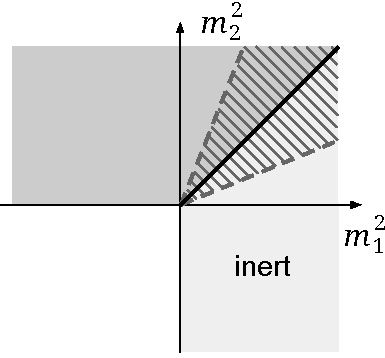
\includegraphics[width=0.3\textwidth]{Figures/i2HDM-space-1.pdf}\hspace{5mm}}
\subfigure[$0 < R < 1$]{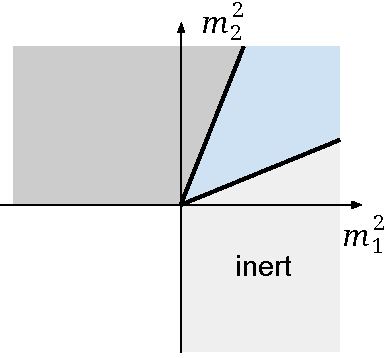
\includegraphics[width=0.3\textwidth]{Figures/i2HDM-space-2.pdf}\hspace{5mm}}
\subfigure[$-1 < R < 0$]{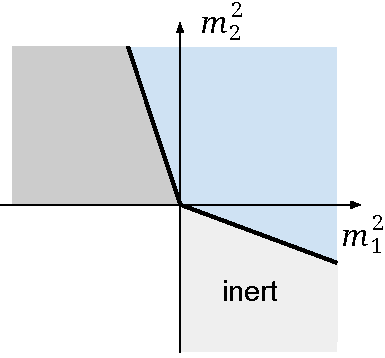
\includegraphics[width=0.3\textwidth]{Figures/i2HDM-space-3.pdf}}
\caption{Restrictions on the $(m_1^2,\, m_2^2)$ plane coming from the requirement that
the inert vacuum is the deepest minimum of the potential. The three cases correspond to (a) $R > 1$,
(b) $0 < R < 1$, (c) $-1 < R < 0$. Light and dark grey correspond to models 
with an inert $v_1 = v,\, v_2 = 0$ and a pseudoinert $v_1 = 0,\, v_2 = v$ vacuum,
respectively, while the blue region in between corresponds to the mixed vacuum,
when both $v_1$ and $v_2$ are non-zero. The dashed region in the left plot indicates coexistence
of the inert and pseudoinert minima at different depths.}
\label{fig:parameter-space}
\end{figure}

Another set of theoretical constraints comes from the symmetry breaking patterns in i2HDM \cite{Deshpande:1977rw}
and from the fact that the potential can have two minima at different depths.
Following \cite{Ginzburg:2010wa},
we introduce $R=\lambda_{345}/2\sqrt{\lambda_1\lambda_2}$,
which satisfies $R> -1$.
Requiring that the inert vacuum corresponds to the global minimum
leads to the following conditions on the parameters of the potential, apart from $m_1^2 > 0$:
\begin{eqnarray}
\label{eq:condition1}
m_2^2 < \frac{\lambda_{345}}{2\lambda_1} m_1^2 = R\, \sqrt{\frac{\lambda_2}{\lambda_1}} m_1^2 \,,&\mbox{if}& |R| < 1\,,\nonumber\\ 
m_2^2 < \sqrt{\frac{\lambda_2}{\lambda_1}} m_1^2 \,, &\mbox{if}& R > 1\,.
\end{eqnarray}
In Fig.~\ref{fig:parameter-space} we visualise these restrictions on the $(m_1^2,\, m_2^2)$ plane
for the three choices of $R$.
The inert, $v_1 = v$, $v_2=0$, and pseudoinert, $v_1 = 0$, $v_2 = v$, vacua can coexist only when $R>1$,
which is shown by the dashed region in Fig.~\ref{fig:parameter-space} (a).
For $R > 1$, the second line in Eq.~(\ref{eq:condition1}) is a stronger condition
than the first line and it guarantees that the inert minimum is the deepest one.
This condition is shown in Fig.~\ref{fig:parameter-space} (a) by the solid black line.

Rewriting  conditions~(\ref{eq:condition1}) for the physical parameters 
we get  the constraint on the Higgs potential in the following compact final form:
\begin{eqnarray}
\label{eq:scalar-pot1}
&&\mbox{the trivial one, } M_{h_1}^2 > 0 \mbox{ for } |R|<1, \\
&&\mbox{and}\nonumber\\
\label{eq:scalar-pot2}
&&M_{h_1}^2 > 
  (\lambda_{345}/2\sqrt{\lambda_1\lambda_2}-1) \sqrt{\lambda_1\lambda_2} v^2
=  (R-1) \sqrt{\lambda_1\lambda_2} v^2 \mbox{ for } R>1,
\end{eqnarray}
where $\lambda_1 \approx 0.129$ is fixed as in the Standard Model by the Higgs mass (\ref{masses}). 
The latter condition places an upper bound on $\lambda_{345}$ for a given DM mass $M_{h_1}$.
